
%	Section 1

\section{Introduction}\label{Section_Introd}
\Headerfooter{Introduction}
\subsection{Neutrino}
\vs\hs
Neutrinos, which are Fermions with spin of 1$/$2, are classified as leptons that do not participate in the strong interaction in the Standard Model (SM) of the particle physics.
Moreover, neutrinos do not have charge.
Therefore, neutrinos interact with other particles only via the weak interaction\footnote{Gravitational interaction can be ignored because gravitational constant (magnitude of the gravitational interaction) is so tiny. Gravitational constant, Fermi coupling constant (magnitude of the weak interaction), fine-structure constant (magnitude of the electromagnetic interaction), and strong coupling constant (magnitude of the strong interaction) are $6.708\,83(15) \times 10^{-39}\,\hbar c\,({\rm GeV}/c^{2})^{-2}$, $1.166\,378\,8(6) \times 10^{-5}\,{\rm GeV}^{-2}$, $7.297\,352\,5693(11) \times 10^{-3}$, and $0.1180(9)$, respectively~\cite{2022Workman}.}, and are difficult to observe.
The name "neutrino" was named by E. Fermi in 1933~\cite{HistoryOfNeutrino}.
The name comes from the "neutral" that means the zero charge, and "ino" that means small in Italian.
Currently, we know that there are three flavors of neutrinos: electron neutrino, muon neutrino, and tau neutrino.\\
\hs
The existence of neutrinos was suggested by W. Pauli in 1930~\cite{HistoryOfNeutrino}.
Once, the energy spectrum of the electron emitted by the beta decay was expected to be the line spectrum.
However, in 1914, J. Chadwick found that the energy spectrum was not the line spectrum but the continuous spectrum~\cite{1914Chadwick}.
To explain the continuous spectrum of the electron reported by Chadwick, Pauli claimed that an unknown particle with spin of 1$/$2 and zero charge is emitted in the beta decay in addition to an electron.
In 1956, more than 20 years after Pauli proposed the existence of neutrinos, (electron anti)neutrinos produced in nuclear reactors were discovered by F. Reines and C. Cowan~\cite{1956Reines}.
In 1962, muon neutrinos were discovered in the accelerator experiment by L. Lederman, M. Schwartz, and J. Steinberger~\cite{1962Danby}.
In 2001, tau neutrinos were discovered in the DONUT (Direct Observation of NU Tau) experiment~\cite{2001Kodama}.





\subsection{Neutrino oscillation}
\vs\hs
In the SM, the neutrino mass was assumed to be zero~\cite{2022Workman}.
However, in 1998, the evidence for the neutrino oscillation was discovered in the Super-Kamiokande and it was proved that the neutrino mass is not zero~\cite{1998Fukuda}.
Neutrino oscillation is a phenomenon that the flavor of neutrino changes while the neutrino passes through a space.\\
\hs
Here, the neutrino oscillation in vacuum is considered.
The flavor eigenstate $\ket{\nu_{\alpha}}$ is represented by the superposition of the mass eigenstate $\ket{\nu_{i}}$,
\begin{eqnarray}
	\ket{\nu_{\alpha}} = \sum_{i=1}^{n} U_{\alpha i}^{*}\ket{\nu_{i}},
\end{eqnarray}
where $n$ ($= 3$) is the number of neutrino species and $U$ is a 3$\,\times\,$3 unitary matrix, called the Pontecorvo-Maki-Nakagawa-Sakata (PMNS) mixing matrix.
This matrix consists of four independent parameters (three mixing angles, $\theta_{12}$, $\theta_{23}$, and $\theta_{13}$, and one phase angle $\delta_{{\rm CP}}$),
\begin{eqnarray}
	U &=& \left(
	\begin{array}{ccc}
		1 & 0       & 0      \\
		0 & c_{23}  & s_{23} \\
		0 & -s_{23} & c_{23}
	\end{array}
	\right)
	\left(
	\begin{array}{ccc}
		c_{13}                        & 0 & s_{13}e^{-i\delta_{{\rm CP}}} \\
		0                             & 1 & 0                             \\
		-s_{13}e^{i\delta_{{\rm CP}}} & 0 & c_{13}
	\end{array}
	\right)
	\left(
	\begin{array}{ccc}
		c_{12}  & s_{12} & 0 \\
		-s_{12} & c_{12} & 0 \\
		0       & 0      & 1
	\end{array}
	\right) \nonumber \\
	&=&\left(
	\begin{array}{ccc}
		c_{12}c_{13}                                           & s_{12}c_{13}                                           & s_{13}e^{-i\delta_{{\rm CP}}} \\
		-s_{12}c_{23}-c_{12}s_{23}s_{13}e^{i\delta_{{\rm CP}}} & c_{12}c_{23}-s_{12}s_{23}s_{13}e^{i\delta_{{\rm CP}}}  & s_{23}c_{13}                  \\
		s_{12}s_{23}-c_{12}c_{23}s_{13}e^{i\delta_{{\rm CP}}}  & -c_{12}s_{23}-s_{12}c_{23}s_{13}e^{i\delta_{{\rm CP}}} & c_{23}c_{13}
	\end{array}
	\right),
\end{eqnarray}
where $c_{ij} \equiv \cos\theta_{ij}$ and $s_{ij} \equiv \sin\theta_{ij}$.
After traveling a distance $L$ ($\simeq ct$ for relativistic neutrinos), the flavor eigenstate evolves as
\begin{eqnarray}
	\ket{\nu_{\alpha}(t)} = \sum_{i=1}^{n} U_{\alpha i}^{*}\ket{\nu_{i}(t)},
\end{eqnarray}
where $\ket{\nu_{i}(t)} = e^{-iE_{i}t}\ket{\nu_{i}(0)}$ ($E_{i}$ is the energy of the neutrino mass eigenstate $\nu_{i}$).
At that time, the probability of being observed as the flavor eigenstate $\ket{\nu_{\beta}}$ is
\begin{eqnarray}\label{Introd_Eq_Prob}
	P_{\alpha\beta} = |\braket{\nu_{\beta}|\nu_{\alpha}(t)}|^{2} = \Bigg|\sum_{i=1}^{n}\sum_{j=1}^{n} U_{\alpha i}^{*}U_{\beta j}\braket{\nu_{j}|\nu_{i}(t)}\Bigg|^{2}.
\end{eqnarray}
Here, neutrinos are relativistic, thus $p_{i} \simeq p_{j} \equiv p \simeq E$. Therefore, $E_{i}$ can be approximated as
\begin{eqnarray}\label{Introd_Eq_E}
	E_{i} = \sqrt{p_{i}^{2}+m_{i}^{2}} = p_{i}\sqrt{1+{m_{i}^{2} \over p_{i}^{2}}} \simeq p_{i}\Bigg(1+{m_{i}^{2} \over 2p_{i}^{2}}\Bigg) \simeq E+{m_{i}^{2} \over 2E}.
\end{eqnarray}
Using Equation (\ref{Introd_Eq_E}) and the orthogonality of the mass eigenstates, $\braket{\nu_{j}|\nu_{i}} = \delta_{ij}$, Equation (\ref{Introd_Eq_Prob}) can be expressed as
\begin{eqnarray}
	P_{\alpha\beta} = \delta_{\alpha\beta}-4\sum_{i<j}^{n} {\rm Re}[U_{\alpha i}U_{\beta i}^{*}U_{\alpha j}^{*}U_{\beta j}]\sin^{2}X_{ij}+2\sum_{i<j}^{n} {\rm Im}[U_{\alpha i}U_{\beta i}^{*}U_{\alpha j}^{*}U_{\beta j}]\sin 2X_{ij},
\end{eqnarray}
where
\begin{eqnarray}\label{Introd_Eq_X}
	X_{ij} = {(m_{i}^{2}-m_{j}^{2})L \over 4E} \equiv {\Delta m_{ij}^{2}L \over 4E} = 1.267{\Delta m_{ij}^{2} \over {\rm eV}^{2}}{L/E \over {\rm m}/{\rm MeV}}.
\end{eqnarray}
\hs
For a simpler example, the neutrino oscillation between two neutrino species in vacuum is considered.
The relationship between flavor eigenstates and mass eigenstates can be expressed as
\begin{eqnarray}\label{Introd_Eq_FlavMass}
	\left(
	\begin{array}{c}
		\ket{\nu_{\alpha}} \\
		\ket{\nu_{\beta}}
	\end{array}
	\right)
	= \left(
	\begin{array}{cc}
		\cos\theta  & \sin\theta \\
		-\sin\theta & \cos\theta
	\end{array}
	\right)
	\left(
	\begin{array}{c}
		\ket{\nu_{1}} \\
		\ket{\nu_{2}}
	\end{array}
	\right)
	= \left(
	\begin{array}{c}
		\cos\theta\ket{\nu_{1}}+\sin\theta\ket{\nu_{2}} \\
		-\sin\theta\ket{\nu_{1}}+\cos\theta\ket{\nu_{2}}
	\end{array}
	\right).
\end{eqnarray}
From Equation~(\ref{Introd_Eq_FlavMass}),
\begin{eqnarray}\label{Introd_Eq_MassFlav}
	\left(
	\begin{array}{c}
		\ket{\nu_{1}} \\
		\ket{\nu_{2}}
	\end{array}
	\right)
	= \left(
	\begin{array}{c}
		\cos\theta\ket{\nu_{\alpha}}-\sin\theta\ket{\nu_{\beta}} \\
		\sin\theta\ket{\nu_{\alpha}}+\cos\theta\ket{\nu_{\beta}}
	\end{array}
	\right).
\end{eqnarray}
Assuming that $\ket{\nu_{\alpha}(0)} = 1$ and $\ket{\nu_{\beta}(0)} = 0$, after traveling a distance $L$ ($\simeq ct$ for relativistic neutrinos), the flavor eigenstates evolve as
\begin{eqnarray}
	\ket{\nu_{\alpha}(t)} &=& \cos\theta\ket{\nu_{1}(t)} + \sin\theta\ket{\nu_{2}(t)} \nonumber \\
	                      &=& \cos\theta \times e^{-iE_{1}t/\hbar}\ket{\nu_{1}(0)} + \sin\theta \times e^{-iE_{2}t/\hbar}\ket{\nu_{2}(0)} \nonumber \\
	                      &=& e^{-iE_{1}t/\hbar}\cos\theta\{\cos\theta\ket{\nu_{\alpha}(0)} - \sin\theta\ket{\nu_{\beta}(0)}\} + e^{-iE_{2}t/\hbar}\sin\theta\{\sin\theta\ket{\nu_{\alpha}(0)} + \cos\theta\ket{\nu_{\beta}(0)}\} \nonumber \\
	                      &=& e^{-iE_{1}t/\hbar}\cos^{2}\theta + e^{-iE_{2}t/\hbar}\sin^{2}\theta, \\
	\ket{\nu_{\beta}(t)}  &=& -\sin\theta\ket{\nu_{1}(t)} + \cos\theta\ket{\nu_{2}(t)} \nonumber \\
	                      &=& -\sin\theta \times e^{-iE_{1}t/\hbar}\ket{\nu_{1}(0)} + \cos\theta \times e^{-iE_{2}t/\hbar}\ket{\nu_{2}(0)} \nonumber \\
	                      &=& -e^{-iE_{1}t/\hbar}\sin\theta\{\cos\theta\ket{\nu_{\alpha}(0)} - \sin\theta\ket{\nu_{\beta}(0)}\} + e^{-iE_{2}t/\hbar}\cos\theta\{\sin\theta\ket{\nu_{\alpha}(0)} + \cos\theta\ket{\nu_{\beta}(0)}\} \nonumber \\
	                      &=& -e^{-iE_{1}t/\hbar}\sin\theta\cos\theta + e^{-iE_{2}t/\hbar}\cos\theta\sin\theta \nonumber \\
	                      &=& \sin\theta\cos\theta(-e^{-iE_{1}t/\hbar} + e^{-iE_{2}t/\hbar}).
\end{eqnarray}
At that time, the probability of being observed as the flavor eigenstate $\ket{\nu_{\beta}}$ is
\begin{eqnarray}
	P_{\alpha\beta} &=& |\braket{\nu_{\beta}(t)|\nu_{\alpha}(0)}|^{2} \nonumber \\
	                &=& |\sin\theta\cos\theta(-e^{iE_{1}t/\hbar} + e^{iE_{2}t/\hbar})(\cos^{2}\theta + \sin^{2}\theta)|^{2} \nonumber \\
	                &=& (\sin\theta\cos\theta)^{2}(-e^{iE_{1}t/\hbar} + e^{iE_{2}t/\hbar})(-e^{-iE_{1}t/\hbar} + e^{-iE_{2}t/\hbar}) \nonumber \\
	                &=& \bigg({1 \over 2}\sin2\theta\bigg)^{2}[2 - \{e^{i(E_{2} - E_{1})t/\hbar} + e^{-i(E_{2} - E_{1})t/\hbar}\}] \nonumber \\
	                &=& {1 \over 4}\sin^{2}2\theta\bigg\{2 - 2\cos{(E_{2} - E_{1})t \over \hbar}\bigg\} \nonumber \\
	                &=& {1 \over 4}\sin^{2}2\theta \times 4\sin^{2}{(E_{2} - E_{1})t \over 2\hbar} \nonumber \\
	                & & \bigg(\because\, 2 - 2\cos{(E_{2} - E_{1})t \over \hbar} = 2 - 2\bigg\{\cos^{2}{(E_{2} - E_{1})t \over 2\hbar} - \sin^{2}{(E_{2} - E_{1})t \over 2\hbar}\bigg\} \nonumber \\
	                & & = 2 - 2\bigg\{1 - 2\sin^{2}{(E_{2} - E_{1})t \over 2\hbar}\bigg\} = 4\sin^{2}{(E_{2} - E_{1})t \over 2\hbar}\bigg) \nonumber \\
	                &=& \sin^{2}2\theta\sin^{2}{(E_{2} - E_{1})t \over 2\hbar} \nonumber \\
	                &=& \sin^{2}2\theta\sin^{2}\bigg({m_{2}^{2} - m_{1}^{2} \over 2E}{ct \over 2\hbar c}\bigg) \,\,\, (\because\,\text{Equation~(\ref{Introd_Eq_E})}) \nonumber \\
	                &=& \sin^{2}2\theta\sin^{2}{\Delta m_{21}^{2}L \over 4E\hbar c} \nonumber \\
	                &=& \sin^{2}2\theta\sin^{2}\bigg({\Delta m_{21}^{2} \over {\rm eV}^{2}}{L/E \over {\rm m}/{\rm eV}}{{\rm eV} \times {\rm m} \over 4 \times 1.9733 \times 10^{-7}}\bigg) \nonumber \\
	                &=& \sin^{2}2\theta\sin^{2}\bigg(1.267{\Delta m_{21}^{2} \over {\rm eV}^{2}}{L/E \over {\rm m}/{\rm MeV}}\bigg) \nonumber \\
	                &=& \sin^{2}2\theta\sin^{2}X_{21} \,\,\, (\because\,\text{Equation~(\ref{Introd_Eq_X})}).
\end{eqnarray}
While the probability of being observed as the flavor eigenstate $\ket{\nu_{\alpha}}$ is
\begin{eqnarray}
	P_{\alpha\alpha} = 1 - \sin^{2}2\theta\sin^{2}X_{21}.
\end{eqnarray}
\hs
Next, the neutrino oscillation between two neutrino species ($\nu_{\rm e}$ and $\nu_{\mu}$) in matter is considered.
In matter, all flavor neutrinos are affected by the potential due to its neutral-current interactions, while only electron neutrinos are affected by the potential due to its charged-current interactions with electrons.
Therefore, Equation~(\ref{Introd_Eq_FlavMass}) and Equation~(\ref{Introd_Eq_MassFlav}) change as
\begin{eqnarray}
	\left(
	\begin{array}{c}
		\ket{\nu_{\rm e}} \\
		\ket{\nu_{\mu}}
	\end{array}
	\right)
	&=& \left(
	\begin{array}{c}
		\cos\theta_{M}\ket{\nu_{1}^{M}}+\sin\theta_{M}\ket{\nu_{2}^{M}} \\
		-\sin\theta_{M}\ket{\nu_{1}^{M}}+\cos\theta_{M}\ket{\nu_{2}^{M}}
	\end{array}
	\right), \\
	\left(
	\begin{array}{c}
		\ket{\nu_{1}^{M}} \\
		\ket{\nu_{2}^{M}}
	\end{array}
	\right)
	&=& \left(
	\begin{array}{c}
		\cos\theta_{M}\ket{\nu_{\rm e}}-\sin\theta_{M}\ket{\nu_{\mu}} \\
		\sin\theta_{M}\ket{\nu_{\rm e}}+\cos\theta_{M}\ket{\nu_{\mu}}
	\end{array}
	\right).
\end{eqnarray}
Assuming that $\ket{\nu_{\rm e}(0)} = 1$ and $\ket{\nu_{\mu}(0)} = 0$, the probability of being observed as the flavor eigenstate $\ket{\nu_{\mu}}$ after traveling a distance $L$ ($\simeq ct$ for relativistic neutrinos) is
\begin{eqnarray}
	P_{{\rm e}\mu} = \sin^{2}2\theta_{M}\sin^{2}X_{M}.
\end{eqnarray}
While the probability of being observed as the flavor eigenstate $\ket{\nu_{\rm e}}$ is
\begin{eqnarray}
	P_{{\rm ee}} = 1 - \sin^{2}2\theta_{M}\sin^{2}X_{M}.
\end{eqnarray}
Here,
\begin{eqnarray}
	M_{1}^{2}           &=&      {m_{1}^{2} + m_{2}^{2} \over 2} + \sqrt{2}G_{F}N_{\rm e}E \label{Introd_Eq_M1} \nonumber \\
	                    & &      - {1 \over 2}\sqrt{(\Delta m_{21}^{2}\sin2\theta)^{2} + (\Delta m_{21}^{2}\cos2\theta - 2\sqrt{2}G_{F}N_{\rm e}E)^{2}}, \\
	M_{2}^{2}           &=&      {m_{1}^{2} + m_{2}^{2} \over 2} + \sqrt{2}G_{F}N_{\rm e}E \nonumber \\
	                    & &      + {1 \over 2}\sqrt{(\Delta m_{21}^{2}\sin2\theta)^{2} + (\Delta m_{21}^{2}\cos2\theta - 2\sqrt{2}G_{F}N_{\rm e}E)^{2}}, \\
	\Delta M_{21}^{2}   &\equiv& M_{2}^{2}-M_{1}^{2} = \sqrt{(\Delta m_{21}^{2}\sin2\theta)^{2} + (\Delta m_{21}^{2}\cos2\theta - 2\sqrt{2}G_{F}N_{\rm e}E)^{2}}, \\
	\sin^{2}2\theta_{M} &=&      \bigg({\Delta m_{21}^{2}\sin2\theta \over \Delta M_{21}^{2}}\bigg)^{2}, \\
	X_{M}               &=&      1.267{\Delta M_{21}^{2} \over {\rm eV}^{2}}{L/E \over {\rm m}/{\rm MeV}}. \label{Introd_Eq_XM}
\end{eqnarray}
In Equation~(\ref{Introd_Eq_M1}) to Equation~(\ref{Introd_Eq_XM}), $M_{1}$ and $M_{2}$ are the effective neutrino masses in matter, $G_{F}$ is the Fermi coupling constant, and $N_{\rm e}$ is the electron number density in the medium.
In a medium with varying density ($N_{\rm e}$), $\sin^{2}2\theta_{M}$ becomes largest when
\begin{eqnarray}
	\Delta m_{21}^{2}\cos2\theta = 2\sqrt{2}G_{F}N_{\rm e}E.
\end{eqnarray}
The effect that the oscillation probability changes significantly with density is called the Mikheyev-Smirnov-Wolfenstein (MSW) effect.
Details about neutrino oscillaitons in matter are summarized in Ref.~\cite{1989Kuo,2022Workman}.\\
\hs
From the above calculation, it can be seen that the neutrino oscillation can be described by six parameters ($\theta_{12}$, $\theta_{23}$, $\theta_{13}$, $\Delta m_{21}^{2}$, $\Delta m_{32}^{2}$, and $\delta_{{\rm CP}}$).
These parameters can be measured by observing the oscillation phenomena of solar neutrinos, atmospheric neutrinos, reactor neutrinos, and accelerator neutrinos.
Table~\ref{Introd_Tab:Neu} shows the three-neutrino mixing parameters and $\delta_{{\rm CP}}$~\cite{PDG}.
Currently, the absolute neutrino masses ($m_{1}$, $m_{2}$, and $m_{3}$) and the neutrino mass ordering are not yet known.
There are two possibilities of the neutrino mass ordering: Normal Ordering (NO, $m_{1}<m_{2}<m_{3}$) or Inverted Ordering (IO, $m_{3}<m_{1}<m_{2}$).
At this time, NO is a little preferred~\cite{2017Abe}.
Moreover, CP conserving points, $\delta_{\rm CP} = 0$ and $\delta_{\rm CP} = \pi$, are rejected at the 95\% confidence level~\cite{2020Abe}.

\begin{table}[h]
	\caption[Three-neutrino mixing parameters and $\delta_{{\rm CP}}$]{
	Three-neutrino mixing parameters and $\delta_{{\rm CP}}$~\cite{PDG}.
	Here, $\theta_{ij}\in[0,\pi/2]$ and $\delta_{{\rm CP}}\in[0,2\pi]$.
	}\label{Introd_Tab:Neu}
	\centering
	\vs
	\begin{tabular}{ll} \hline \hline
		$\sin^{2}\theta_{12}$     & $0.307 \pm 0.013$                                 \\
		$\sin^{2}\theta_{23}$ (NO)& $0.547\,^{+0.018}_{-0.024}$                       \\
		$\sin^{2}\theta_{23}$ (IO)& $0.534\,^{+0.021}_{-0.024}$                       \\
		$\sin^{2}\theta_{13}$     & $(2.20 \pm 0.07) \times 10^{-2}$                  \\
		$\Delta m_{21}^{2}$       & $(7.53 \pm 0.18) \times 10^{-5}\,{\rm eV}^{2}$    \\
		$\Delta m_{32}^{2}$ (NO)  & $(2.437 \pm 0.033) \times 10^{-3}\,{\rm eV}^{2}$  \\
		$\Delta m_{32}^{2}$ (IO)  & $(-2.519 \pm 0.033) \times 10^{-3}\,{\rm eV}^{2}$ \\
		$\delta_{\rm CP}$         & $1.23 \pm 0.21\,\pi\,{\rm rad}$                   \\ \hline \hline
	\end{tabular}
\end{table}





\subsection{Neutrinos from core-collapse supernovae}
\vs\hs
A star with mass more than about eight solar masses causes a huge explosion called "core-collapse supernova" at the end of its life~\cite{1988Hirata,2013Burrows}.
The released energy is approximately $10^{53}~{\rm ergs}$, and about 99\% of that energy is carried away by neutrinos~\cite{1990Burrows}.
Here, observations of neutrinos from core-collapse supernovae are briefly described.

\subsubsection{Neutrinos from SN1987A}\label{Subsubsec_SN1987A}
\vs\hs
On February 23, 1987, Kamiokande II, IMB (Irvine-Michigan-Brookhaven), and Baksan observed a burst of neutrinos from SN1987A\footnote{Mont Blanc also reported neutrino signals from SN1987A~\cite{1990Bethe}. However, signals reported in Mont Blanc were unrelated to SN1987A.}, which is a core-collapse supernova that occurred in the Large Magellanic Cloud~\cite{1987Hirata,1987Bionta,1987Alekseev}.
Here, Kamiokande II and IMB are water Cherenkov detectors and Baksan is a scintillator detector.
Figure~\ref{Introd_KamIMB} shows the neutrino events from SN1987A observed in Kamiokande II and IMB~\cite{1988Hirata}.
This was the world's first observation of neutrinos from a supernova (neutrinos from outside the solar system), and we got a better understanding on supernovae from this observation~\cite{1990Bethe}.
To further understand about supernovae, detectors around the world, including Super-Kamiokande, are waiting for the next neutrino burst from nearby supernova.

\begin{figure}[H]
	\centering
	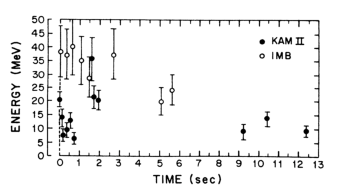
\includegraphics[width=9cm]{Figures/Introduction/KamIMB}
	\caption[Neutrino events from SN1987A observed in Kamiokande II and IMB]{
	Neutrino events from SN1987A observed in Kamiokande II and IMB~\cite{1988Hirata}.
	}\label{Introd_KamIMB}
\end{figure}

\subsubsection{Diffuse supernova neutrino background}
\vs\hs
As described in Section~\ref{Subsubsec_SN1987A}, now we are waiting for the next neutrino burst from nearby supernova.
However, according to Ref.~\cite{2013Adams}, a galactic core-collapse supernova rate is only $3.2^{+7.3}_{-2.6}$ per century, and actually bursts of neutrinos from supernovae have not been observed since SN1987A.
Nevertheless, there is a way to understand about supernovae without waiting for the neutrino bursts.
Neutrinos emitted from all past core-collapse supernovae comprise an integrated flux called the diffuse supernova neutrino background (DSNB)~\cite{2010Beacom}.
Detecting the DSNB would contribute to our understanding of the mechanism of supernova explosions and the history of star formation.\\
\hs
According to Ref.~\cite{2015Nakazato}, the DSNB flux on the Earth can be described as
\begin{eqnarray}
	{d\Phi(E_{\nu}) \over dE_{\nu}} &=& c\int_{0}^{z_{\rm max}} {dz \over H_{0}\sqrt{\Omega_{m}(1 + z)^{3} + \Omega_{\Lambda}}} \nonumber \\
	                                & & \times\Bigg[R_{\rm CC}(z)\int_{0}^{Z_{\rm max}} \psi_{\rm ZF}(z, Z)\Bigg\{\int_{M_{\rm min}}^{M_{\rm max}} \psi_{\rm IMF}(M){dN(M, Z, E^{\prime}_{\nu}) \over dE^{\prime}_{\nu}}dM\Bigg\}dZ\Bigg],
\end{eqnarray}
where $c$ is the velocity of light, $H_{0} = 70\,{\rm km}\,{\rm s}^{-1}\,{\rm Mpc}^{-1}$, $\Omega_{m} = 0.3$, $\Omega_{\Lambda} = 0.7$, $Z$ is the metallicity of progenitors, $M$ is the initial mass of progenitors, and $dN(M, Z, E^{\prime}_{\nu})/dE^{\prime}_{\nu}$ is the neutrino number spectrum from the core collapse of a progenitor including the neutrino oscillation effect.
The neutrino energy on the Earth $E_{\nu}$ is related to that at the redshift $z$, $E^{\prime}_{\nu}$, as $E^{\prime}_{\nu} = (1 + z)E_{\nu}$.
The total core-collapse rate $R_{\rm CC}(z)$ is determined by the cosmic star formation rate density.
The metallicity distribution function of progenitors $\psi_{\rm ZF}(z, Z)$ and the initial mass function of progenitors $\psi_{\rm IMF}(M)$ are normalized as
\begin{eqnarray}
	\int_{0}^{Z_{\rm max}} \psi_{\rm ZF}(z, Z)dZ = 1, \\
	\int_{M_{\rm min}}^{M_{\rm max}} \psi_{\rm IMF}(M)dM = 1.
\end{eqnarray}
Figure~\ref{Introd_DSNBpred} shows the predictions of DSNB $\bar{\nu}_{\rm e}$ flux~\cite{2021Abe}.
As shown in this figure, the predicted DSNB $\bar{\nu}_{\rm e}$ fluxes differ by more than one order of magnitude between the smallest one and the largest one.

\begin{figure}[p]
	\centering
	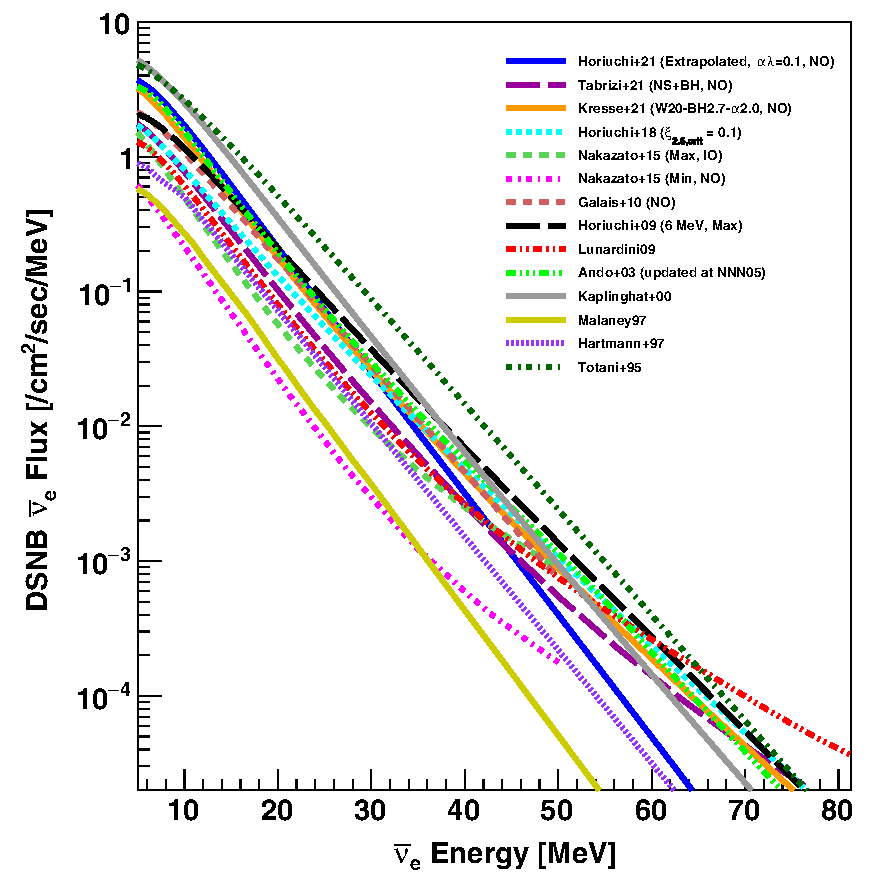
\includegraphics[width=8cm]{Figures/Introduction/DSNBpred}
	\caption[Predictions of DSNB $\bar{\nu}_{\rm e}$ flux]{
	Predictions of DSNB $\bar{\nu}_{\rm e}$ flux~\cite{2021Abe}.
	These fluxes are predicted by theoretical models of 
	Horiuchi~$+$~21~\cite{2021Horiuchi}, Tabrizi~$+$~21~\cite{2021Tabrizi}, Kresse~$+$~21~\cite{2021Kresse},
	Horiuchi~$+$~18~\cite{2018Horiuchi}, Nakazato~$+$~15~\cite{2015Nakazato}, Galais~$+$~10~\cite{2010Galais},
	Horiuchi~$+$~09~\cite{2009Horiuchi}, Lunardini09~\cite{2009Lunardini}, Ando~$+$~03~\cite{2003Ando}, Kaplinghat~$+$~00~\cite{2000Kaplinghat},
	Malaney~$+$~97~\cite{1997Malaney}, Hartmann~$+$~97~\cite{1997Hartmann}, and Totani~$+$~95~\cite{1995Totani}.
	Ando~$+$~03 model was updated at the NNN05 conference~\cite{2005Ando}.
	Details of each theoretical model are summarized in Ref.~\cite{2021Abe,2023HaradaPhD}.
	}\label{Introd_DSNBpred}
\end{figure}





\subsection{DSNB search}\label{Subsec_DSNBsearch}
\vs\hs
As shown in Figure~\ref{Introd_DSNBpred}, there are many predictions of DSNB $\bar{\nu}_{\rm e}$ flux.
Observation of the DSNB can limit these predictions.
Here, the DSNB search method and the current status of DSNB search are explained.\\
\hs
Most of experiments look for the inverse-beta decay (IBD) events by electron antineutrinos ($\ibd$) in the DSNB search.
It is because its cross section is large in the $\mathcal{O}$(10) MeV region, as shown in Figure~\ref{Introd_EffNeuCroSec}, where the DSNB flux is large.

%\begin{figure}[p]
%	\centering
%	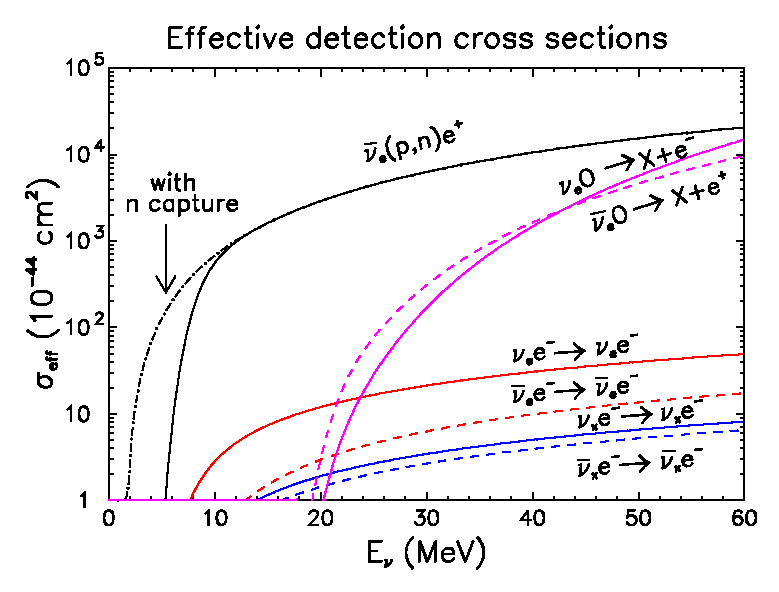
\includegraphics[width=10cm]{Figures/Introduction/EffNeuCroSec}
%	\caption[Effective neutrino interaction cross sections including energy resolution and threshold effects in large water Cherenkov detectors]{
%	Effective neutrino interaction cross sections including energy resolution and threshold effects in large water Cherenkov detectors~\cite{2005Fogli}.
%	Horizontal axis shows the neutrino energy.
%	}\label{Introd_EffNeuCroSec}
%\end{figure}

\begin{figure}[p]
	\centering
	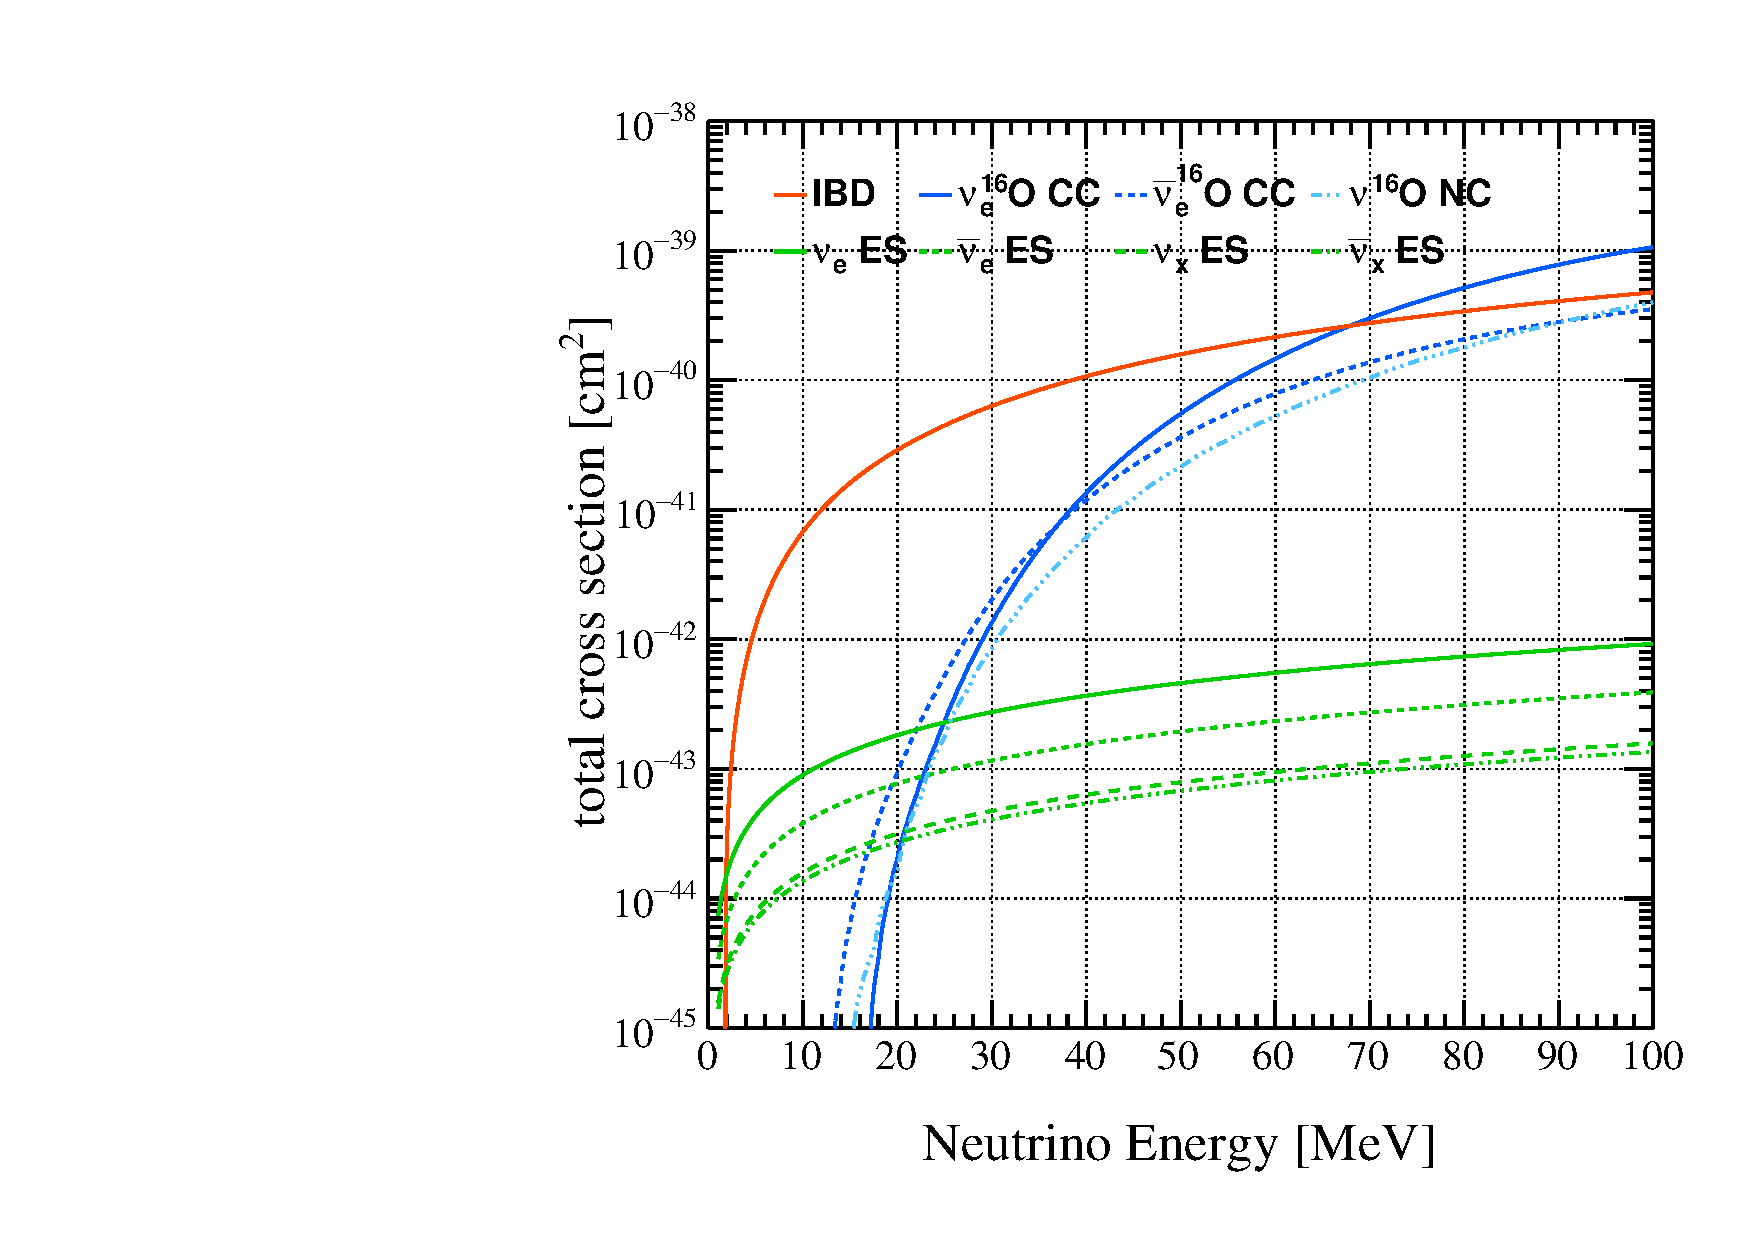
\includegraphics[width=8cm]{Figures/Introduction/Nakanishi_XS}
	\caption[Neutrino interaction cross sections]{
	Neutrino interaction cross sections~\cite{2023NakanishiMas}.
	CC, NC, and ES stand for charged-current interactions, neutral-current interactions, and elastic scattering reactions, respectively.
	}\label{Introd_EffNeuCroSec}
\end{figure}

\hs
Since the 1980s, the DSNB search has been performed in various experiments.
The DSNB has not been observed yet, but the upper limits of $\bar{\nu}_{\rm e}$ flux are approaching and arriving at the predicted DSNB $\bar{\nu}_{\rm e}$ fluxes.
Figure~\ref{Introd_DSNB_Upper} shows the upper limits of $\bar{\nu}_{\rm e}$ flux in recent DSNB searches~\cite{2023Ando}.
Here, we focus on the DSNB search performed in Super-Kamiokande (SK), KamLAND, and Borexino.

%\begin{figure}[tbp]
%	\centering
%	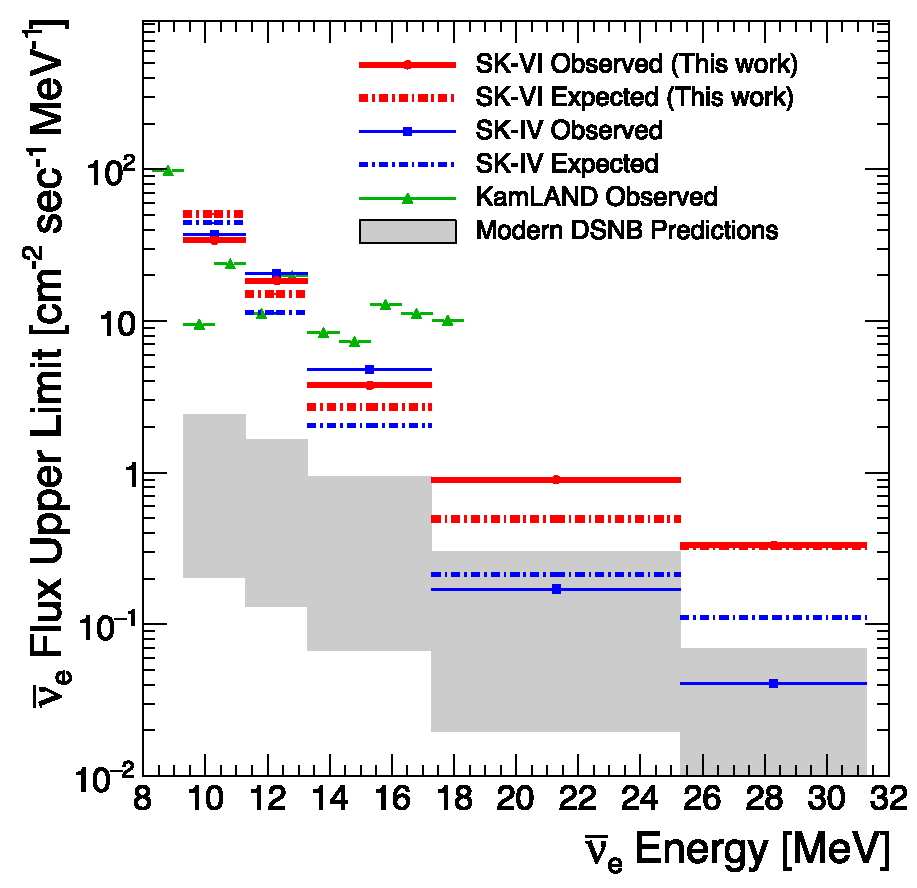
\includegraphics[width=8cm]{Figures/Introduction/SK-VI_DSNB_Upper}
%	\caption[Upper limit of $\bar{\nu}_{\rm e}$ flux in the SK-Gd DSNB search]{
%	Upper limit of $\bar{\nu}_{\rm e}$ flux in the SK-Gd DSNB search~\cite{2023Harada}.
%	Solid lines show the observed 90\%-confidence level upper limit for SK-VI (red)~\cite{2023Harada}, SK-IV (blue)~\cite{2021Abe}, and KamLAND (green)~\cite{2022AbeKamLAND}, respectively.
%	Dashed-dot lines show the expected 90\%-confidence level upper limit for SK-VI (red)~\cite{2023Harada} and SK-IV (blue)~\cite{2021Abe}, respectively.
%	Gray-shaded region shows the predictions of DSNB $\bar{\nu}_{\rm e}$ flux~\cite{2022Ekanger,2021Horiuchi,2021Tabrizi,2021Kresse,2018Horiuchi,2015Nakazato,2010Galais,2009Horiuchi,2009Lunardini,2003Ando,2000Kaplinghat,1997Malaney,1997Hartmann}.
%	Ando~$+$~03 model was updated at the NNN05 conference~\cite{2005Ando}.
%	}\label{Introd_SK-VI_DSNB_Upper}
%\end{figure}

\begin{figure}[tbp]
	\centering
	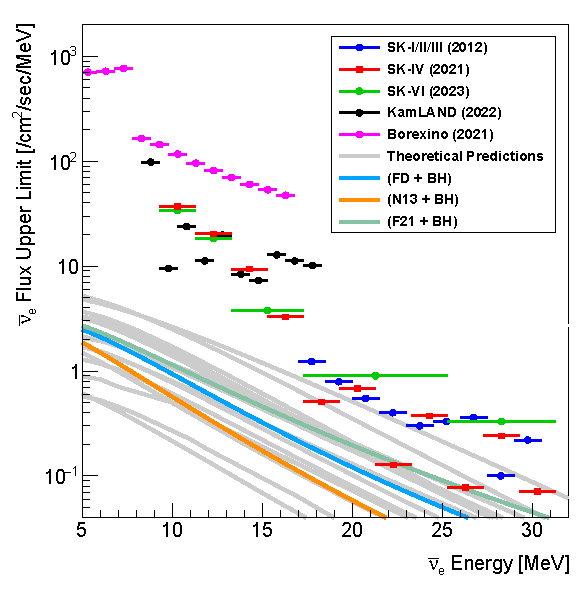
\includegraphics[width=8cm]{Figures/Introduction/DSNB_Upper}
	\caption[Upper limits of $\bar{\nu}_{\rm e}$ flux in recent DSNB searches]{
	Upper limits of $\bar{\nu}_{\rm e}$ flux in recent DSNB searches~\cite{2023Ando}.
	Plots show the 90\%-confidence level upper limits for SK-I/II/III (blue)~\cite{2012Abe}, SK-IV (red)~\cite{2021Abe}, SK-VI (green)~\cite{2023Harada}, KamLAND (black)~\cite{2022AbeKamLAND}, and Borexino (magenta)~\cite{2021Agostini}, respectively.
	Lines show the theoretical predictions of DSNB $\bar{\nu}_{\rm e}$ flux.
	FD, BH, N13, and F21 stand for Fermi-Dirac, black hole, Nakazato (2013)~\cite{2013Nakazato}, and Fornax (2021)~\cite{2021Burrows,2021Nakagura}, respectively.
	}\label{Introd_DSNB_Upper}
\end{figure}

\hs
SK is a 50-kilotons water Cherenkov detector in Kamioka, Gifu, Japan.
Details of the SK are described in Section~\ref{Section_SK}.
In 2012, the DSNB search using 2,853~days of data was performed in SK.
This search gave the upper limits of $\bar{\nu}_{\rm e}$ flux in the neutrino energy region above 17.3~MeV~\cite{2012Abe}.
Moreover, in 2008, the data acquisition system was renewed (see Section~\ref{subsec_data_acqu}).
As a result, in addition to the positron signal generated by the IBD reaction, the signal of a 2.2~MeV gamma-ray generated by neutron capture on free proton in water also became available (see Figure~\ref{Introd_DSNB_SK}).

\begin{figure}[h]
	\centering
	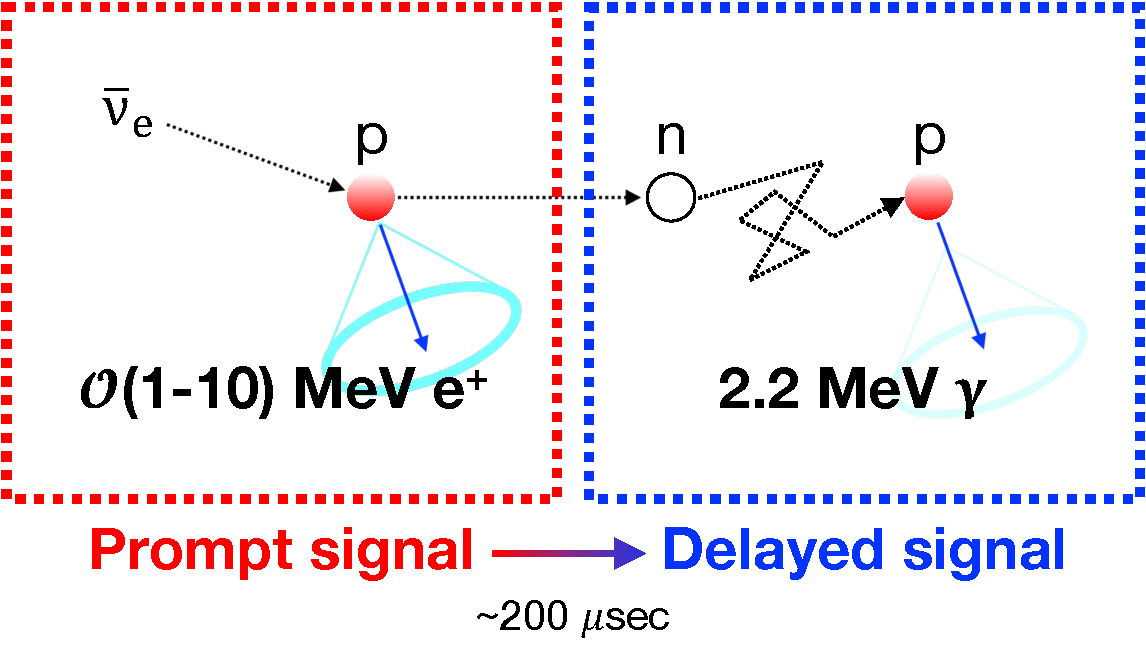
\includegraphics[width=8cm]{Figures/Introduction/DSNB_SK}
	\caption[Schematic view of a DSNB event in SK]{
	Schematic view of a DSNB event in SK.
	The positron emits Cherenkov photons immediately, while the neutron is thermalized and then captured on free proton in water, emitting a 2.2~MeV gamma-ray.
	The gamma-ray give their energy to electrons or positrons via Compton scattering or pair production, then Cherenkov photons are emitted.
	}\label{Introd_DSNB_SK}
\end{figure}

By detecting the positron signal (prompt signal) and the neutron signal (delayed signal), a large number of backgrounds that do not contain neutrons can be removed, and the DSNB search in the lower energy region became possible.
However, the 2.2~MeV gamma-rays are low-energy events in SK.
Therefore, the neutron-tagging efficiency is low ($\sim$20\%), and the statistics become small.
In 2021, the DSNB search with the prompt and delayed signals using 2,970~days of data was performed in SK.
This search gave the upper limits of $\bar{\nu}_{\rm e}$ flux in the neutrino energy region above 9.3~MeV~\cite{2021Abe}.
Furthermore, in 2020, 0.011\% by mass of gadolinium (Gd) was loaded in the SK detector to improve the neutron-tagging efficiency, and the Super-Kamiokande Gadolinium (SK-Gd) experiment started~\cite{2022Abe,2004Beacom}.
Details of the SK-Gd experiment are described in Section~\ref{SK_Obs_pha}.
In 2023, the DSNB search using 552.2~days of data with 0.011\% gadolinium-loaded water was performed in SK-Gd.
The upper limits of $\bar{\nu}_{\rm e}$ flux in this search is comparable to that in SK DSNB search using 2,970~days of pure-water data~\cite{2023Harada}.\\
\hs
KamLAND is a 1-kilotons liquid scintillator detector in Kamioka, Gifu, Japan.
The advantage of KamLAND is that the 2.2~MeV gamma-ray generated by neutron capture on free proton can be detected with an efficiency of about 100\%.
In 2022, the DSNB search using 4,528.5~days of data was performed in KamLAND.
This search gave the upper limits of $\bar{\nu}_{\rm e}$ flux in the neutrino energy region from 8.3~MeV to 30.8~MeV~\cite{2022AbeKamLAND}.
Especially, the upper limits are the most stringent below 12.3~MeV.\\
\hs
Borexino is a 278-tons liquid scintillator detector in Gran Sasso, Italy.
The strength of Borexino is that the energy threshold is low thanks to the extremely low radiopurity.
In 2021, the DSNB search using 2,771~days of data was performed in Borexino.
This search gave the upper limits of $\bar{\nu}_{\rm e}$ flux in the neutrino energy region from 1.8~MeV to 16.8~MeV~\cite{2021Agostini}.
The upper limits below 8.3~MeV are given only by Borexino.

%The positron emits Cherenkov photons immediately, while the neutron is thermalized and then captured on gadolinium, emitting a total of about 8~MeV of gamma-rays.





\subsection{NCQE background in SK-Gd DSNB search}\label{Subsec_NCQEbackground}
\vs\hs
As described in Section~\ref{Subsec_DSNBsearch}, a large number of backgrounds that do not contain neutrons can be removed by detecting prompt and delayed signals.
However, backgrounds that contain neutrons cannot be completely removed.
One of the main backgrounds in the SK-Gd DSNB search is caused by the atmospheric neutrino-oxygen neutral-current quasielastic (NCQE) scattering reactions.
Figure~\ref{DSNB_NCQE} shows the schematic view of a DSNB event and a NCQE event in SK-Gd.
NCQE reactions can be expressed as
\begin{eqnarray}
	\nu(\bar{\nu})\,+\,^{16}{\rm O}\,&\to&\,\nu(\bar{\nu})\,+\,^{15}{\rm O}\,+\,\gamma\,+\,{\rm n}, \nonumber \\
	\nu(\bar{\nu})\,+\,^{16}{\rm O}\,&\to&\,\nu(\bar{\nu})\,+\,^{15}{\rm N}\,+\,\gamma\,+\,{\rm p},
\end{eqnarray}
where the atmospheric neutrino knocks out a nucleon of the oxygen nucleus, and the residual nucleus may emit one or more de-excitation gamma-rays with a few MeV.
When a neutron is knocked out, the combination of de-excitation gamma-rays and neutron mimics the DSNB event, making it difficult to distinguish between NCQE and DSNB events.
Therefore, the precise estimation of NCQE events is essential for the DSNB discovery in SK-Gd.

\begin{figure}[h]
	\centering
	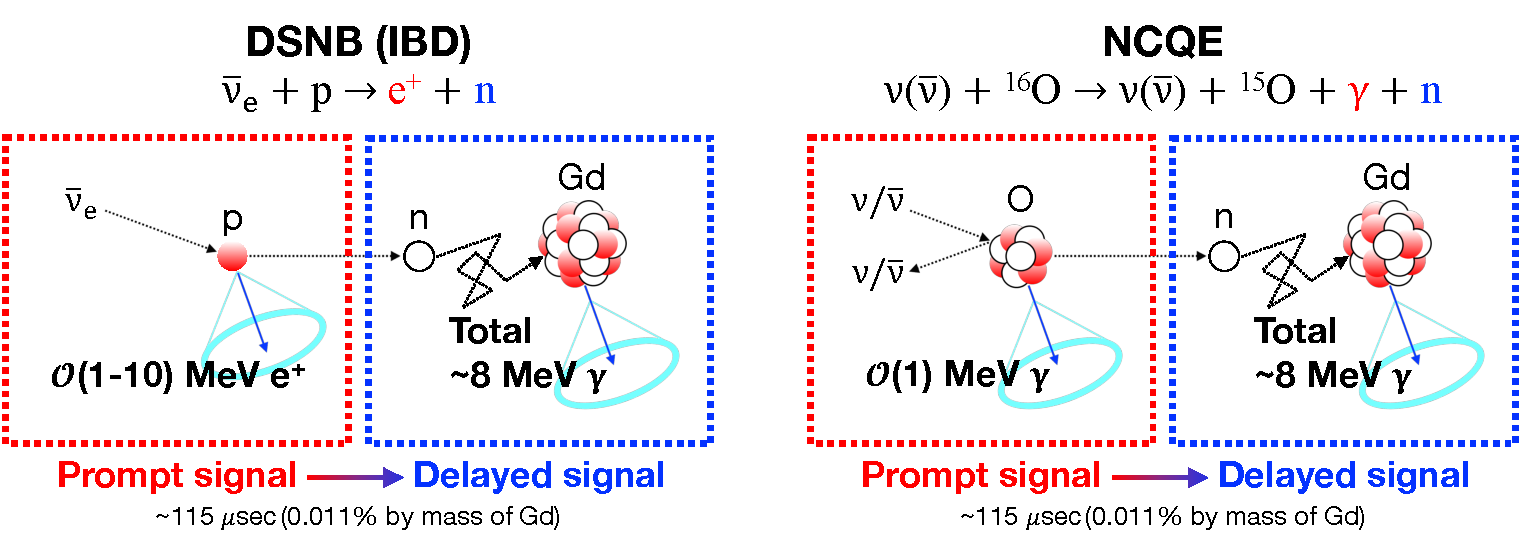
\includegraphics[width=16cm]{Figures/Introduction/DSNB_NCQE}
	\caption[Schematic view of a DSNB event and a NCQE event in SK-Gd]{
	Schematic view of a DSNB event (left) and a NCQE event (right) in SK-Gd.
	}\label{DSNB_NCQE}
\end{figure}

\hs
To estimate the NCQE events precisely, the behavior of neutrons in water must be understood.
Figure~\ref{DSNB_NCQE_n} shows the kinetic energy of neutrons in DSNB events and NCQE events.
In DSNB events, the outgoing neutron has at most a few MeV, while in NCQE events, the knocked-out neutron may have hundreds of MeV.
In the latter case, it can knock out other nucleons of oxygen nuclei in water, and additional de-excitation gamma-rays and neutrons are generated.
Since the numbers of gamma-rays and neutrons affect the event reconstruction, it is crucial to understand the nucleon-nucleus interactions in water (secondary interactions).
Detailed schematic view of a NCQE event is shown in Figure~\ref{Introd_NCQE_PriSec}.

\begin{figure}[h]
	\centering
	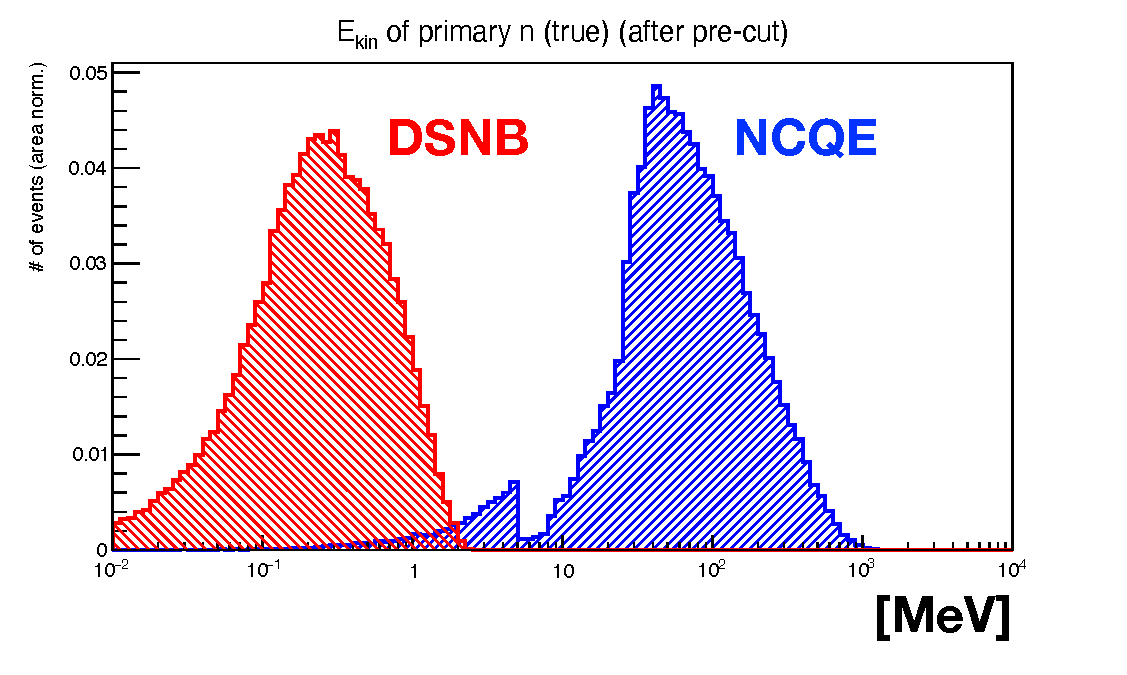
\includegraphics[width=10cm]{Figures/Introduction/DSNB_NCQE_n}
	\caption[Kinetic energy of neutrons in DSNB events and NCQE events]{
	Kinetic energy of neutrons in DSNB events and NCQE events.
	This figure was made by using MC.
	}\label{DSNB_NCQE_n}
\end{figure}

\begin{figure}[h]
	\centering
	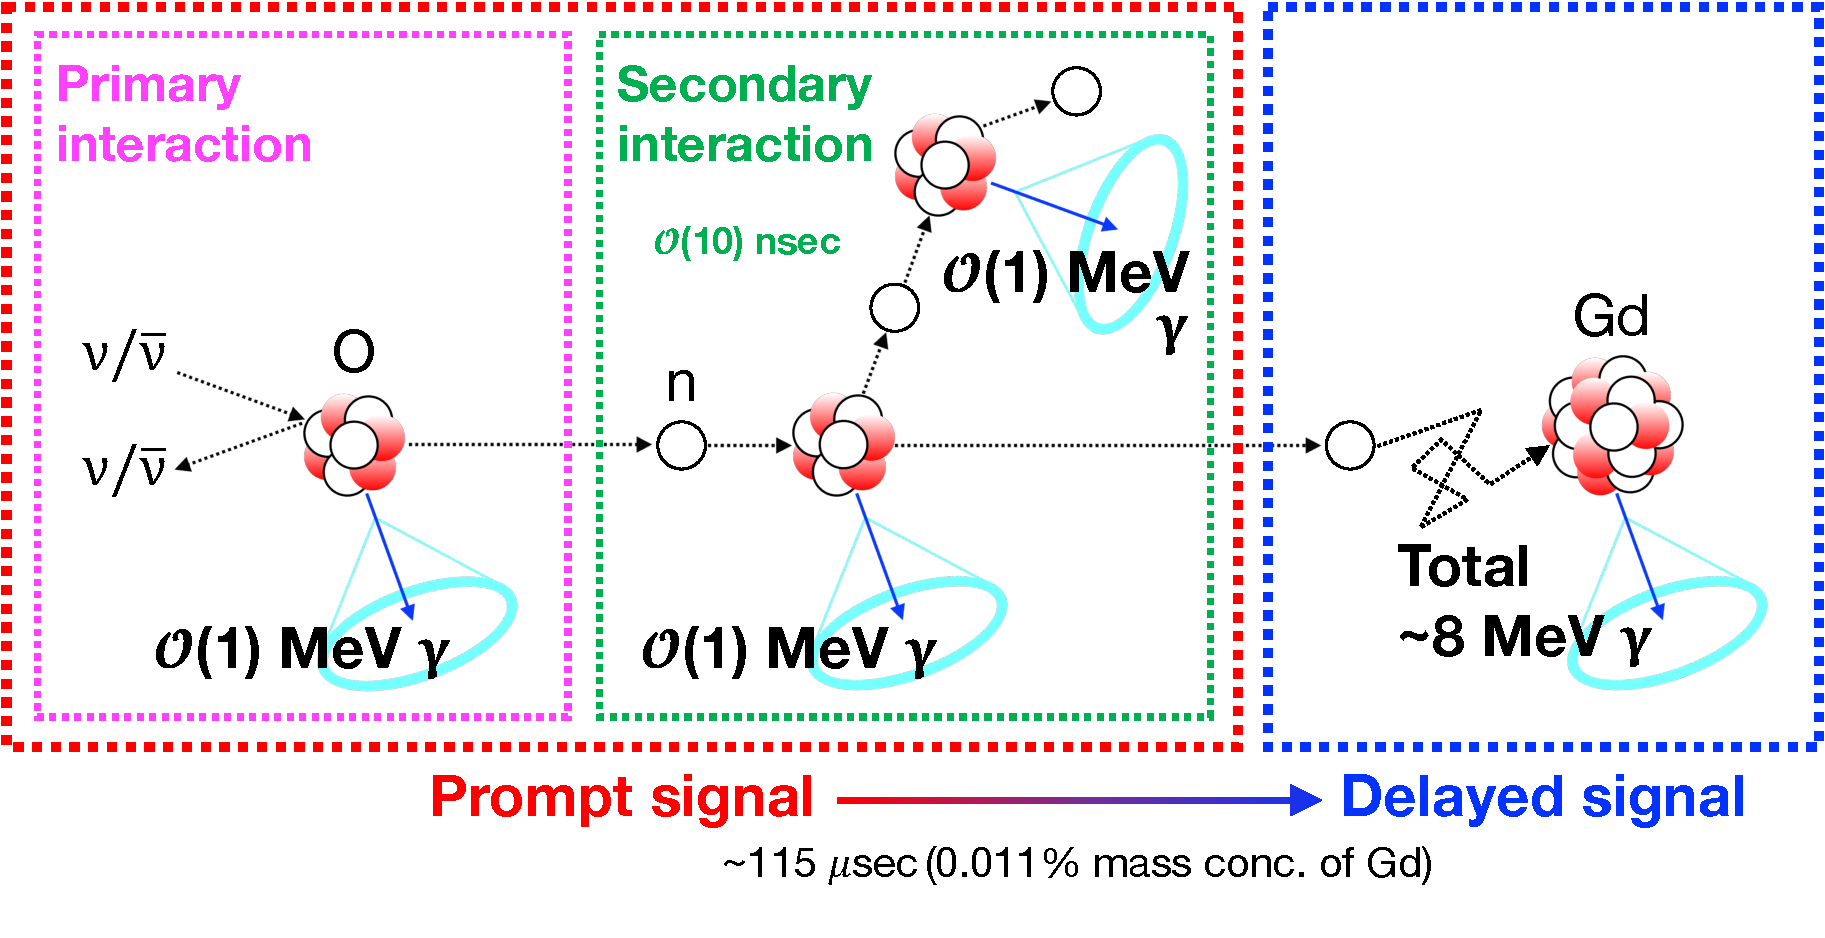
\includegraphics[width=12cm]{Figures/Introduction/NCQE_PriSec}
	\caption[Detailed schematic view of a NCQE event]{
	Detailed schematic view of a NCQE event.
	Prompt signal consists of gamma-rays generated by neutrino-nucleus (primary) interaction and nucleon-nucleus (secondary) interaction.
	}\label{Introd_NCQE_PriSec}
\end{figure}

\hs
Figure~\ref{Harada_DSNB} shows the reconstructed energy spectra of the observed data and the expected backgrounds in the SK-Gd DSNB search~\cite{2023Harada}.
In this figure, the cyan color-filled histogram shows the expected number of NCQE background events and the hatched areas show the total systematic uncertainty for each bin.
In this search, systematic uncertainty on the NCQE events is taken as 68\%~\cite{2023HaradaPhD}, which is too large to discover the DSNB in the near future.
Each component of the systematic uncertainty on the NCQE events in the SK-Gd DSNB search is summarized in Table~\ref{Introd_Tab:SystNCQE}~\cite{2023HaradaPhD}.
From this table, we can confirm that uncertainties of T2K cross section, neutron multiplicity, and spectral shape are dominant.
Uncertainties of neutron multiplicity and spectral shape are related to the number of neutrons and gamma-rays generated by secondary interactions, respectively.
Moreover, uncertainty of T2K cross section, which is used to scale the number of NCQE events, mainly comes from the gamma-rays by secondary interactions.
Figure~\ref{Harada_DSNB} and Table~\ref{Introd_Tab:SystNCQE} show how important it is to understand secondary interactions.
Details of T2K cross section are described in Section~\ref{Subsec_MeasurementsNCQE}.

\begin{figure}[h]
	\centering
	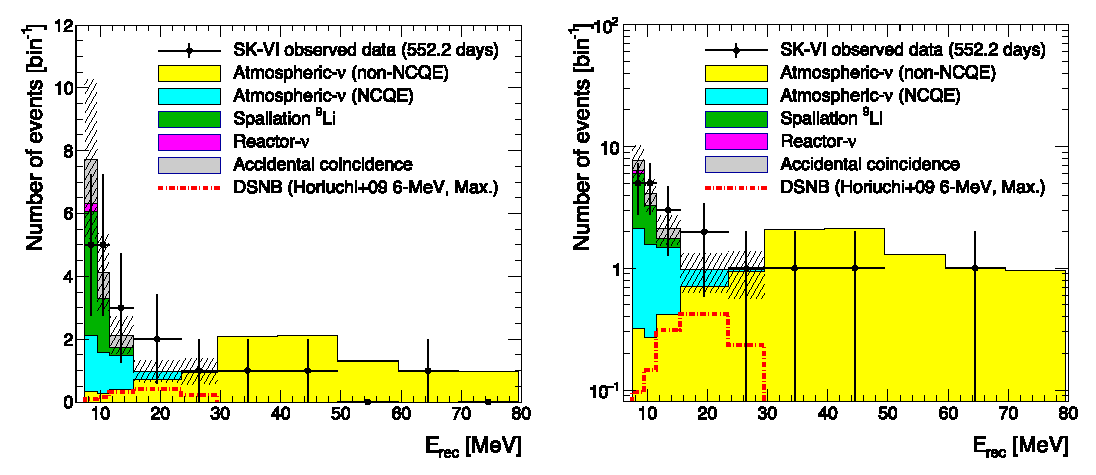
\includegraphics[width=14cm]{Figures/Introduction/Harada_DSNB}
	\caption[Reconstructed energy spectra of the observed data and the expected backgrounds in the SK-Gd DSNB search]{
	Reconstructed energy spectra of the observed data and the expected backgrounds in the SK-Gd DSNB search~\cite{2023Harada}.
	Left and right figure shows in a linear and a logarithmic scale for the vertical axis, respectively.
	These figures include not only the DSNB search window ([7.49, 29.49]~MeV) but also the side-band region above 29.49 MeV.
	Each color-filled histogram shows the expected number of backgrounds, and these background histograms are stacked on the other histograms.
	Details of these backgrounds are described later.
	The hatched areas show the total systematic uncertainty for each bin.
	The red dashed-dot line shows the expected number of DSNB events predicted by the Horiuchi~$+$~09 model~\cite{2009Horiuchi}.
	}\label{Harada_DSNB}
\end{figure}

\begin{table}[h]
	\caption[Systematic uncertainty on the NCQE events in the SK-Gd DSNB search]{
	Systematic uncertainty on the NCQE events in the SK-Gd DSNB search~\cite{2023HaradaPhD}.
	This table is the same as TABLE~9.2 in Ref.~\cite{2023HaradaPhD}.
	}\label{Introd_Tab:SystNCQE}
	\centering
	\vs
	\begin{tabular}{lc} \hline \hline
		T2K cross section          & 44\% \\
		Atmospheric neutrino flux  & 15\% \\
		Flux difference            & 7\%  \\
		Reductions                 & 2\%  \\
		Neutron tagging efficiency & 9\%  \\
		Neutron multiplicity       & 30\% \\
		Spectral shape             & 37\% \\ \hline
		Total                      & 68\% \\ \hline \hline
	\end{tabular}
\end{table}





\subsection{Measurements of NCQE cross section}\label{Subsec_MeasurementsNCQE}
\subsubsection{Measurements using accelerator neutrinos}
\vs\hs
In Table~\ref{Introd_Tab:SystNCQE}, uncertainty of T2K cross section is estimated by using the result of accelerator neutrino-oxygen NCQE cross section measurement in the T2K experiment~\cite{2019Abe}.
In this measurement, data from a $14.94(16.35) \times 10^{20}$ protons-on-target exposure of the neutrino (antineutrino) beam was used, and the flux-averaged NCQE-like cross sections on oxygen nuclei were measured to be
\begin{eqnarray}
	\langle \sigma_{\rm \nu\mathchar`-NCQE} \rangle       &=& 1.70 \pm 0.17({\rm stat.}) ^{+0.51}_{-0.38}({\rm syst.}) \times 10^{-38}\,{\rm cm}^{2}/{\rm oxygen}, \label{Introd_Eq_nuNCQE} \\
	\langle \sigma_{\rm \bar{\nu}\mathchar`-NCQE} \rangle &=& 0.98 \pm 0.16({\rm stat.}) ^{+0.26}_{-0.19}({\rm syst.}) \times 10^{-38}\,{\rm cm}^{2}/{\rm oxygen}, \label{Introd_Eq_nubNCQE}
\end{eqnarray}
where $\langle \sigma_{\rm \nu\mathchar`-NCQE} \rangle$ is for neutrinos at a flux-averaged energy of 0.82~GeV and $\langle \sigma_{\rm \bar{\nu}\mathchar`-NCQE} \rangle$ is for antineutrinos at a flux-averaged energy of 0.68~GeV.
The result of (\ref{Introd_Eq_nuNCQE}) was consistent with that of the previous NCQE cross section measurement in T2K ($\langle \sigma_{\rm \nu\mathchar`-NCQE} \rangle = 1.55\,^{+0.71}_{-0.35}({\rm stat.} \oplus {\rm syst.}) \times 10^{-38}\,{\rm cm}^{2}/{\rm oxygen}$), where data from a $3.01 \times 10^{20}$ protons-on-target exposure of the neutrino beam was used~\cite{2014Abe}.
The 44\% T2K cross section uncertainty in Table~\ref{Introd_Tab:SystNCQE} can be estimated by using (\ref{Introd_Eq_nuNCQE}) and (\ref{Introd_Eq_nubNCQE}),
\begin{eqnarray}
	\sqrt{\Bigg\{\sqrt{\bigg({0.17 \over 1.70}\bigg)^{2} + \bigg({0.51 \over 1.70}\bigg)^{2}}\Bigg\}^{2} + \Bigg\{\sqrt{\bigg({0.16 \over 0.98}\bigg)^{2} + \bigg({0.26 \over 0.98}\bigg)^{2}}\Bigg\}^{2}} \sim 44\%.
\end{eqnarray}
\hs
The large uncertainty mainly comes from the gamma-rays by secondary interactions.
Figure~\ref{Introd_T2K_thetaC} shows the reconstructed Cherenkov angle ($\theta_{\rm C}$) distributions from the FHC (neutrino-mode) sample and the RHC (antineutrino-mode) sample in the T2K NCQE cross section measurement~\cite{2019Abe}.
$\theta_{\rm C}$ is related to the number of gamma-rays, and $\theta_{\rm C}$ becomes larger as the number of gamma-rays by secondary interactions gets larger.
In Figure~\ref{Introd_T2K_thetaC}, we can confirm that, in the case of the FHC sample, there is a large discrepancy between data and MC in high $\theta_{\rm C}$ region where events with multiple gamma-rays are dominant.
This means that more gamma-rays are generated by secondary interactions in MC, that is, the agreements of the secondary interaction model used in MC is poor.

\begin{figure}[h]
	\centering
	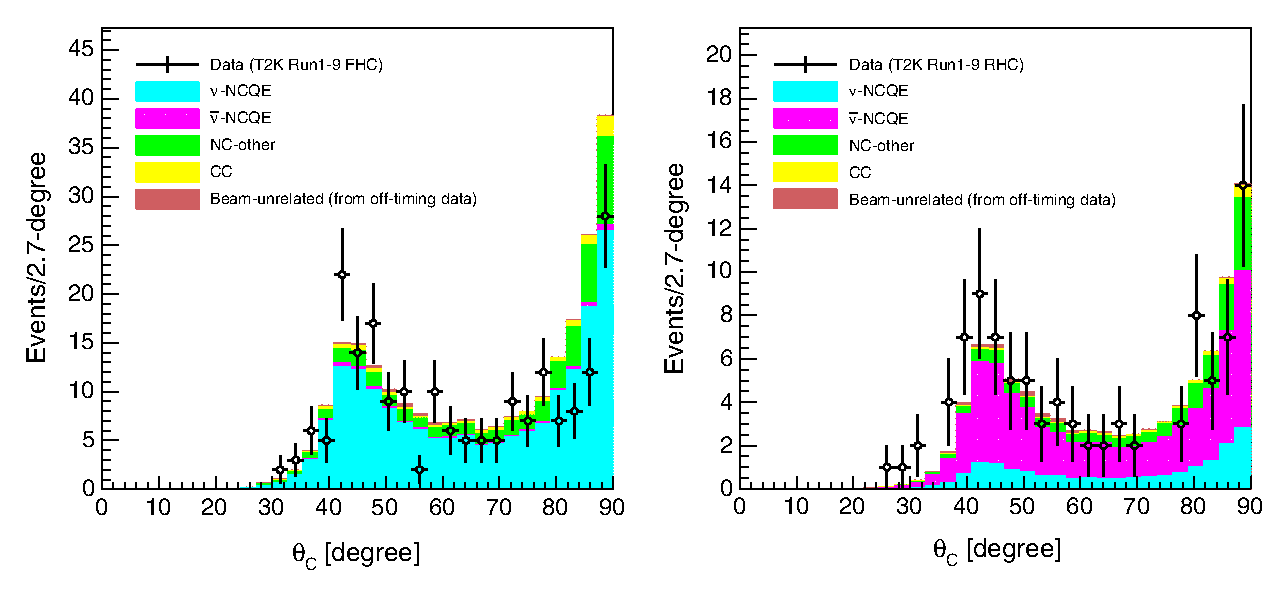
\includegraphics[width=14cm]{Figures/Introduction/T2K_thetaC}
	\caption[Reconstructed Cherenkov angle ($\theta_{\rm C}$) distributions from the FHC (neutrino-mode) sample and the RHC (antineutrino-mode) sample in T2K NCQE cross section measurement]{
	Reconstructed Cherenkov angle ($\theta_{\rm C}$) distributions from the FHC (neutrino-mode) sample (left) and the RHC (antineutrino-mode) sample (right) in the T2K NCQE cross section measurement~\cite{2019Abe}.
	In the left figure, there is a large discrepancy between data and MC in high $\theta_{\rm C}$ region where events with multiple gamma-rays are dominant.
	}\label{Introd_T2K_thetaC}
\end{figure}

\subsubsection{Measurements using atmospheric neutrinos}
\vs\hs
It is important to measure the NCQE cross section using atmospheric neutrinos, which are the source of backgrounds in the DSNB search, and to confirm the consistency with the NCQE cross section measurements using accelerator neutrinos.
The first measurement of the atmospheric neutrino-oxygen NCQE cross section was performed in SK pure water phase~\cite{2019Linyan}.
In this measurement, 2,778~days of SK pure water data from October 2008 to October 2017 was used, and the flux-averaged NCQE cross section on oxygen nuclei was measured to be
\begin{eqnarray}
	\langle \sigma_{\rm NCQE} \rangle = 1.01 \pm 0.17({\rm stat.}) ^{+0.78}_{-0.30}({\rm syst.}) \times 10^{-38}\,{\rm cm}^{2}/{\rm oxygen}.
\end{eqnarray}
Figure~\ref{Introd_Linyan_NCQE} shows the measured NCQE cross section~\cite{2019Linyan}, the theoretical NCQE cross section~\cite{2012Ankowski}, and the atmospheric neutrino flux measured in SK~\cite{2016Richard}.
The large uncertainty in this measurement also mainly comes from the gamma-rays and neutrons by secondary interactions.

\begin{figure}[h]
	\centering
	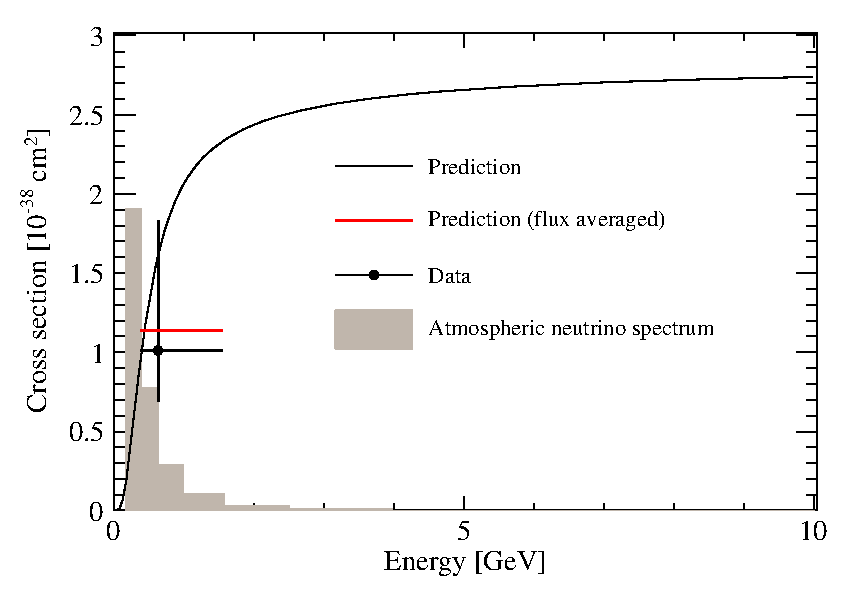
\includegraphics[width=10cm]{Figures/Introduction/Linyan_NCQE}
	\caption[The measured NCQE cross section, the theoretical NCQE cross section, and the atmospheric neutrino flux measured in SK]{
	The measured NCQE cross section~\cite{2019Linyan}, the theoretical neutrino-oxygen NCQE cross section~\cite{2012Ankowski}, and the atmospheric neutrino flux measured in SK~\cite{2016Richard}.
	}\label{Introd_Linyan_NCQE}
\end{figure}

\subsubsection{Issues in previous measurements}
\hs
In the NCQE cross section measurements described above, the large uncertainty mainly came from secondary interactions.
A more precise secondary interaction model is required to reduce the uncertainty, but, so far, the secondary interaction model based on the Bertini Cascade model (BERT)~\cite{2015Wright} was the only choice in MC.
However, now other secondary interaction models like the Binary Cascade model (BIC)~\cite{2004Folger} and the Li$\grave{\text{e}}$ge Intranuclear Cascade model (INCL++)~\cite{2013Boudard} can be employed and compared with data.
In Section~\ref{Sec_Model}, the reproducibility of the observed data in each secondary interaction model using atmospheric neutrino events is discussed.\\
\hs
Moreover, the measurement of the neutrino-oxygen NCQE cross section had not been performed in SK-Gd.
The NCQE cross section measurement in SK-Gd would contribute to our understanding of the behavior of neutrons in water, as well as the performance of the SK-Gd experiment.
In Section~\ref{Sec_NCQE}, the first measurement of the atmospheric neutrino-oxygen NCQE cross section in the Gd-loaded SK water Cherenkov detector is reported.\\





%\begin{figure}[tbp]
%	\centering
%	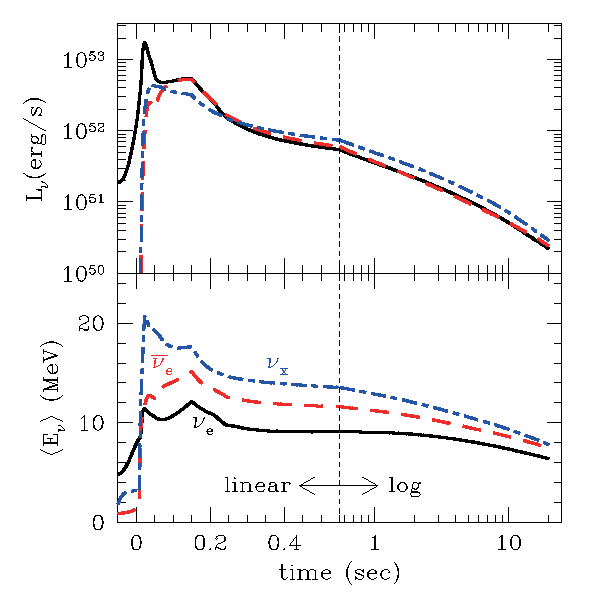
\includegraphics[width=8cm]{Figures/Introduction/TimeLE}
%	\caption[Time evolution of the luminosity and average energy of neutrinos]{
%	Time evolution of the luminosity and average energy of neutrinos~\cite{2013Nakazato}.
%	}\label{Introd_TimeLE}
%\end{figure}





\newpage

